% topic Template for ME3023 - Measurements in Mechanincal Systems - Tennessee Technological University
%
% Spring 2020 - Summer 2020 - Fall 2022
% Tristan Hill, May 31, 2020
% Demonstration 1 - Dimensional Instruments
% Topic 1 - Using Calipers

\documentclass{beamer}                         % for presentation (has nav buttons at bottom)
%\documentclass[handout]{beamer}  % for handout 
\usepackage{beamerthemesplit}
\usepackage{amsmath}
\usepackage{listings}
\usepackage{multicol}
\usepackage{framed}

\beamertemplateballitem

\definecolor{TTUpurple}{rgb}{0.3098, 0.1607, 0.5176} % TTU Purple (primary)
\definecolor{TTUgold}{rgb}{1.0000, 0.8666, 0.0000} % TTU Gold (primary)

\setbeamercolor{palette primary}{bg=TTUpurple,fg=TTUgold}
\setbeamercolor{palette secondary}{bg=black,fg=TTUgold}
\setbeamercolor{palette tertiary}{bg=black,fg=TTUpurple}
\setbeamercolor{palette quaternary}{bg=TTUgold,fg=black}
\setbeamercolor{structure}{fg=TTUpurple} % itemize, enumerate, etc
\setbeamercolor{section in toc}{fg=TTUpurple} % TOC sections

% custom colors 
\definecolor{mygray}{rgb}{.6, .6, .6}
\definecolor{mypurple}{rgb}{0.6,0.1961,0.8}
\definecolor{mybrown}{rgb}{0.5451,0.2706,0.0745}
\definecolor{mygreen}{rgb}{0, .39, 0}
\definecolor{mypink}{rgb}{0.9960, 0, 0.9960}

% color commands
\newcommand{\R}{\color{red}}
\newcommand{\B}{\color{blue}}
\newcommand{\BR}{\color{mybrown}}
\newcommand{\K}{\color{black}}
\newcommand{\G}{\color{mygreen}}
\newcommand{\PR}{\color{mypurple}}
\newcommand{\PN}{\color{mypink}}
\newcommand{\GD}{\color{TTUgold}}
\newcommand{\OR}{\color{orange}}

\newcommand{\Lagr}{\mathcal{L}} % lagrangian

\newcommand{\vspccc}{\vspace{6mm}\\} % large vertical space
\newcommand{\vspcc}{\vspace{4mm}\\}   % medium vertical space
\newcommand{\vspc}{\vspace{2mm}\\}     % small vertical space

\newcommand{\hspcccc}{\hspace{10mm}} % large horizontal space
\newcommand{\hspccc}{\hspace{6mm}} % large horizontal space
\newcommand{\hspcc}{\hspace{4mm}}   % medium horizontal space
\newcommand{\hspc}{\hspace{2mm}}     % small horizontal space


\author{ME3023 - Measurements in Mechanical Systems} % original formatting from Mike Renfro, September 21, 2004

\newcommand{\DNUM}{1\hspace{2mm}} % Demonstration number
\newcommand{\TNUM}{1\hspace{2mm}} % Topic number  ->  (4th Topic)
\newcommand{\demotitle}{Dimensional Instruments }
\newcommand{\topictitle}{Using Calipers} 

\newcommand{\sectiontitleI}{Overview}
\newcommand{\sectiontitleII}{Components}
\newcommand{\sectiontitleIII}{Vernier Calipers}
\newcommand{\sectiontitleIV}{Digital Calipers}
\newcommand{\sectiontitleV}{Group Activity}


\title{Topic \DNUM - \demotitle}

\date{Mechanical Engineering\vspc Tennessee Technological University}

\begin{document}

\lstset{language=MATLAB,basicstyle=\ttfamily\small,showstringspaces=false}

\frame{\titlepage \center\begin{framed}\Large \textbf{Topic \TNUM - \topictitle}\end{framed} \vspace{5mm}}

% Section 0: Outline
	\frame{

		\large \textbf{Topic \TNUM - \topictitle} \vspace{3mm}\\

		\begin{itemize}
			\item \sectiontitleI	\vspc % Section I
			\item \sectiontitleII 	\vspc % Section II
			\item \sectiontitleIII 	\vspc %Section III
			\item \sectiontitleIV 	\vspc %Section IV
			\item \sectiontitleV 	\vspc %Section V
		\end{itemize}

	}

% Section I:
\section{\sectiontitleI}

	\frame{
		\frametitle{\sectiontitleI}

		\begin{itemize}

		\item A caliper ( ... a pair of calipers) is a device used to measure the distance between two opposite sides of an object. {\tiny Text: \href{https://en.wikipedia.org/wiki/Calipers}{Wikipedia}}
		\begin{itemize}

			\item Length, Width, Height
			\item Inside and Outside Diameter
			\item Depth 

		\end{itemize}

		\vspace{5mm}
		\item There is a wide variety of caliper(s). This word means different things in different fields. 
		\begin{itemize}

			\item Engineering and Deisgn
			\item Machining and Construction
			\item Medical Applications and Others

		\end{itemize}
		\item

		\end{itemize}

	}


% Section II:
\section{\sectiontitleII}

	\frame{
		\frametitle{\sectiontitleII}

		{\tiny Text: \href{https://en.wikipedia.org/wiki/Vernier_scale}{Wikipedia}}

		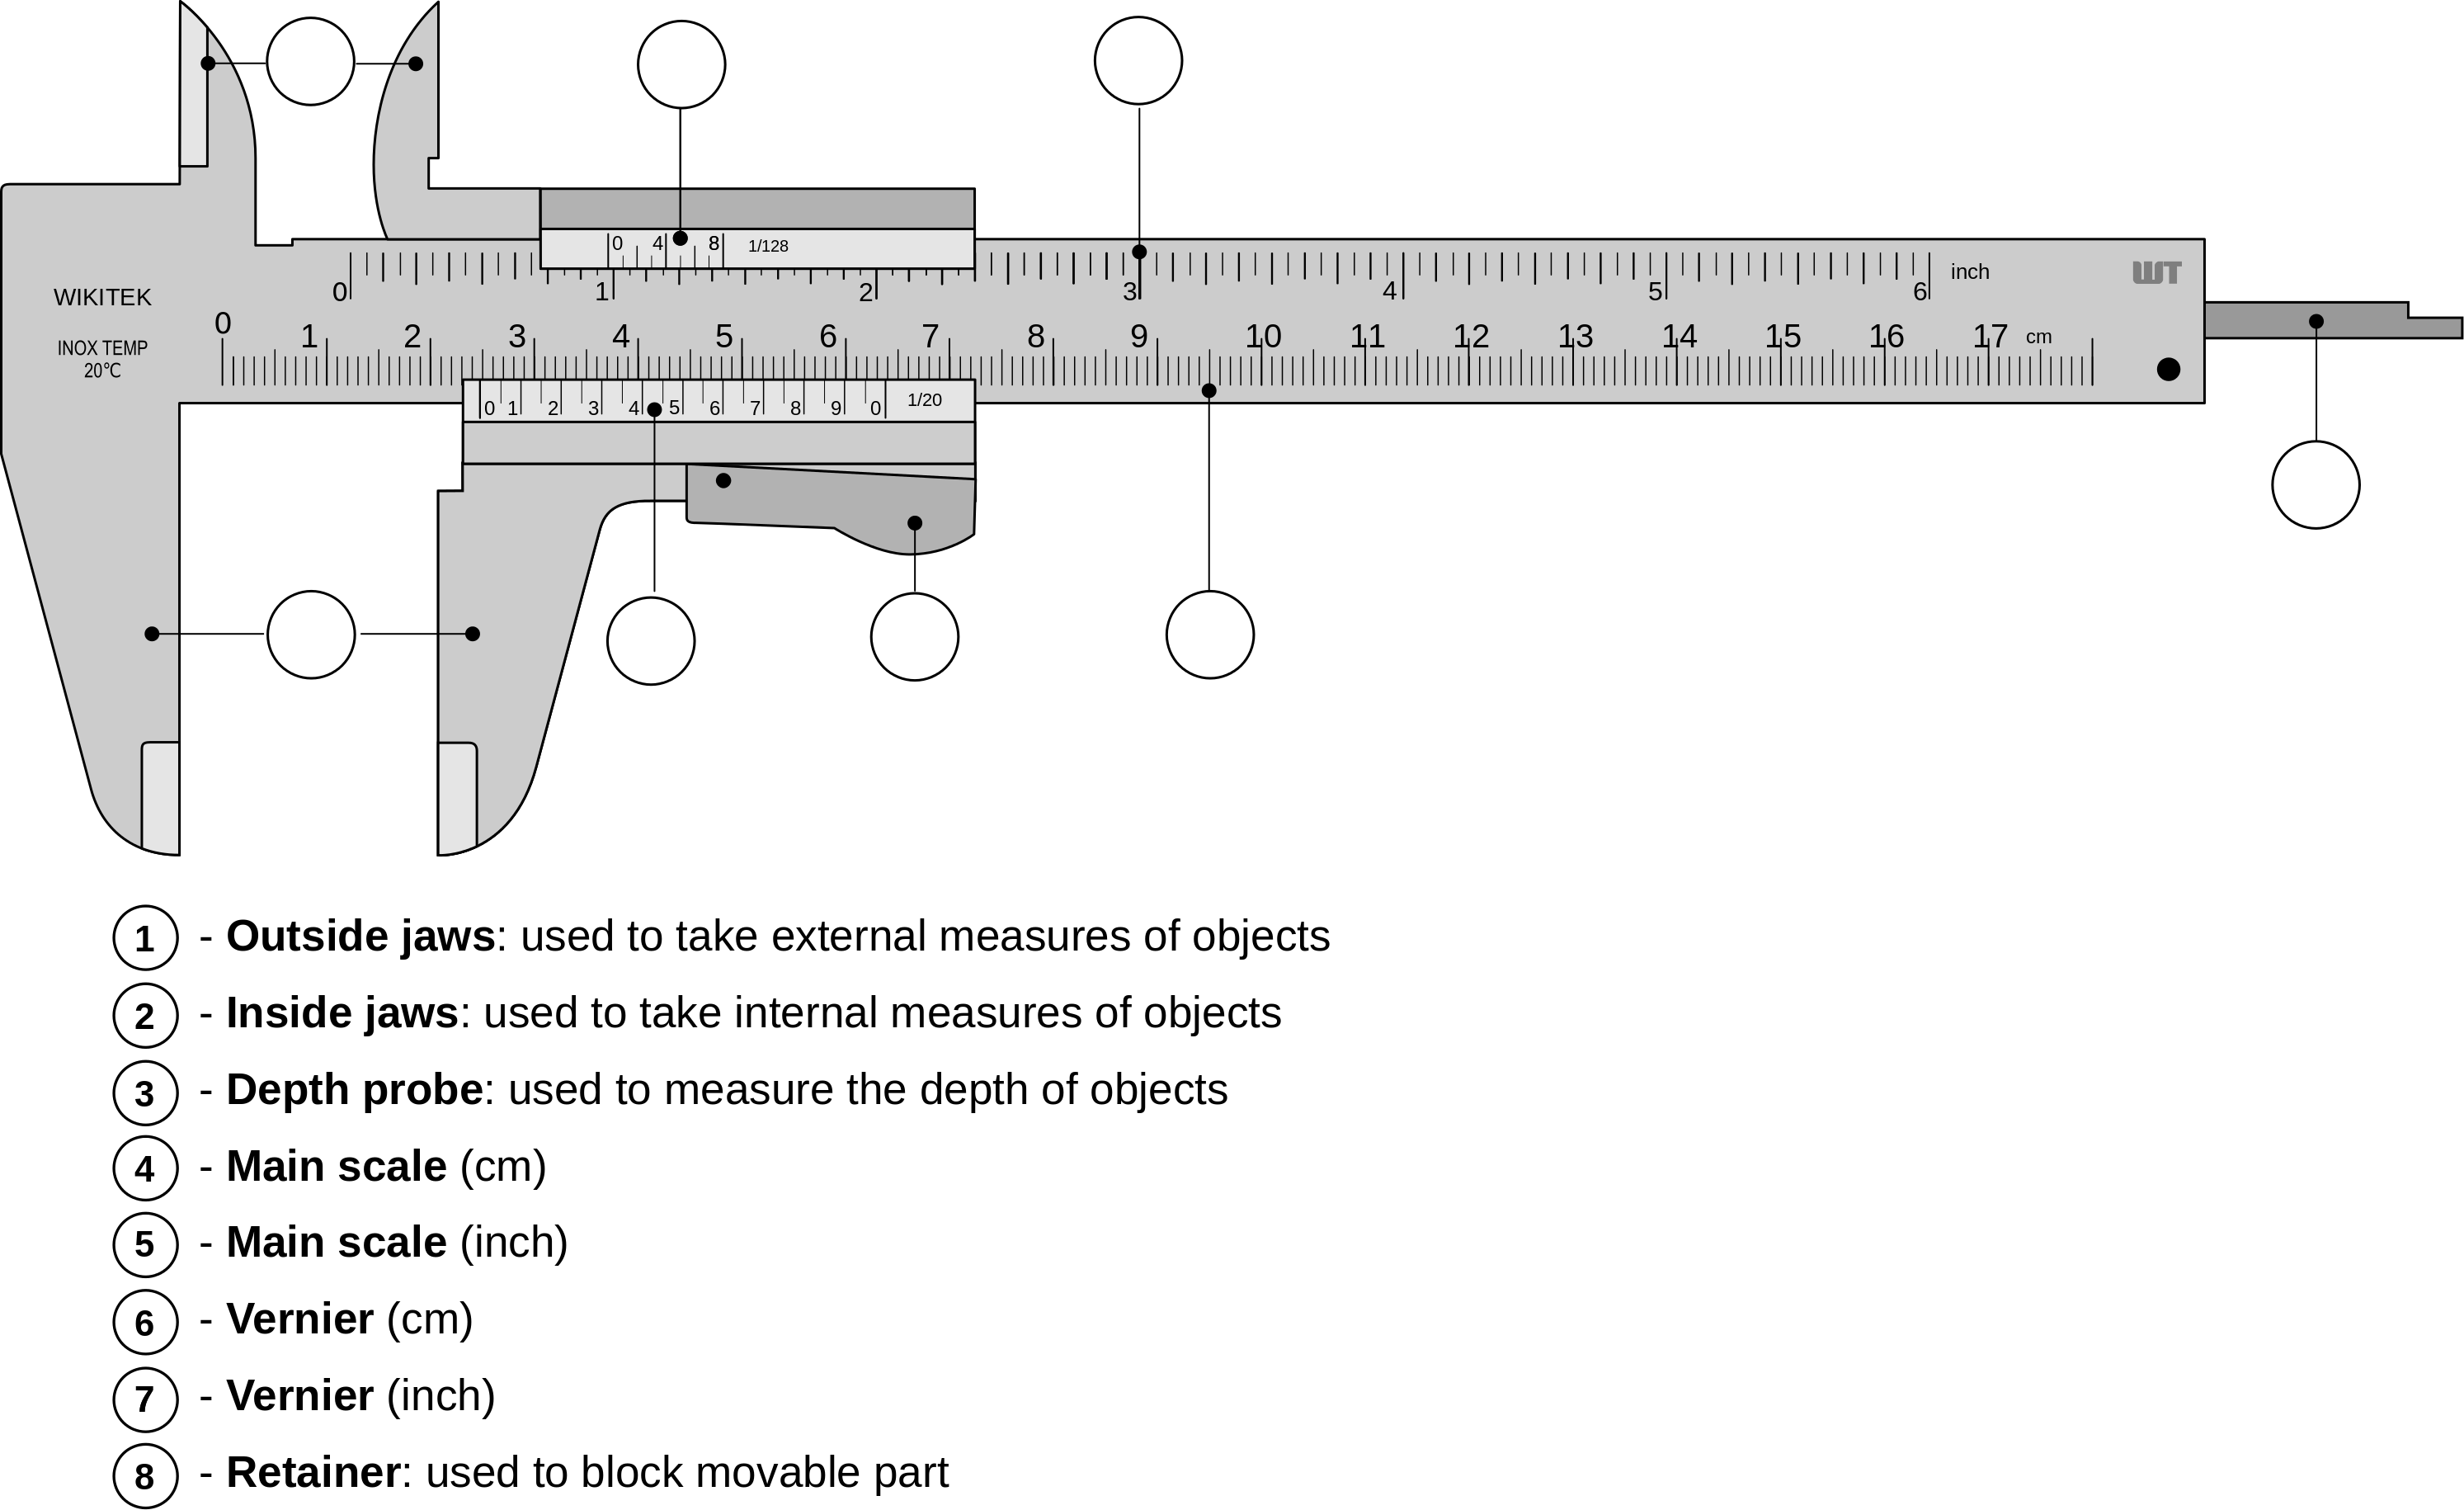
\includegraphics[scale=.08]{calipers_fig1.png}

	}



% Section III:
\section{\sectiontitleIII}


	\frame{
		\frametitle{\sectiontitleIII}
		\scriptsize	

		A vernier scale is a visual aid to take an accurate measurement reading between two graduation markings on a linear scale by using mechanical interpolation; thereby increasing resolution and reducing measurement uncertainty by using Vernier acuity to reduce human estimation error. \vspc

		\includegraphics[scale=.07]{vernier_calipers_fig1_cropped.png}

	}


	\frame{
		\frametitle{\sectiontitleIII}
		\scriptsize
		\begin{multicols}{2}
			\begin{enumerate}
				\item Inspect the jaws. Wipe the jaws with a clean rag or cloth. \vspcc

				\item Close the jaws around the object gently and avoid deflecting the object. Verify the reading is zero. \vspcc

				\item Read the main scale and record the measurement. \vspcc

				\item Read the Vernier scale and add to the main scale measurement. \vspace{8mm}\\
		    \end{enumerate}


			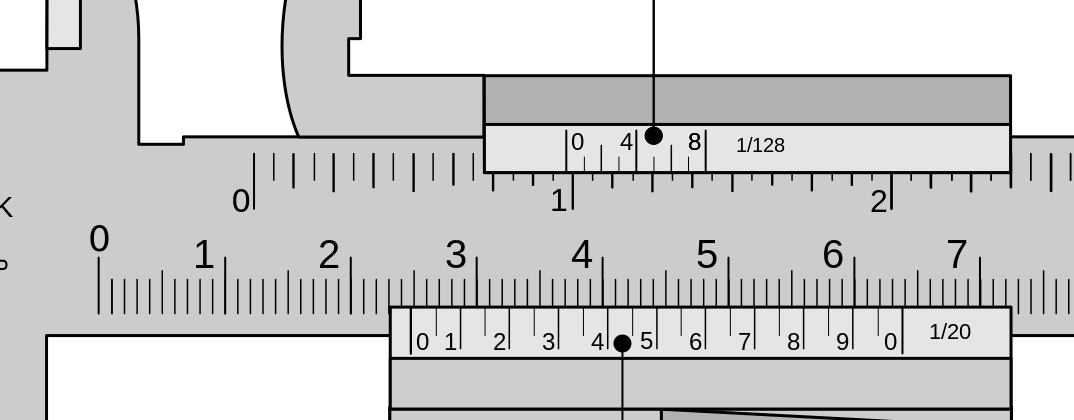
\includegraphics[scale=.15]{calipers_fig1_cropped.png}
		\end{multicols}
	}


% Section IV:
\section{\sectiontitleIV}

	
	\frame{
		\frametitle{\sectiontitleIV}

		A digital caliper contains an embedded processor and user interface to facilitate the measurement process.

		\includegraphics[scale=.08]{digital_calipers_fig1_cropped.png}

	}	


	\frame{
		\frametitle{\sectiontitleIV}
		\scriptsize

		\begin{multicols}{2}
			\begin{enumerate}
				\item Inspect the jaws. Wipe the jaws with a clean rag or cloth.
				\item Close the jaws around the object gently and avoid deflecting the object. Verify the reading is zero.
				\item If needed, press the button to zero the tool.
				\item Read the output and record the measurement. \vspace{5mm}\\
		    \end{enumerate}

			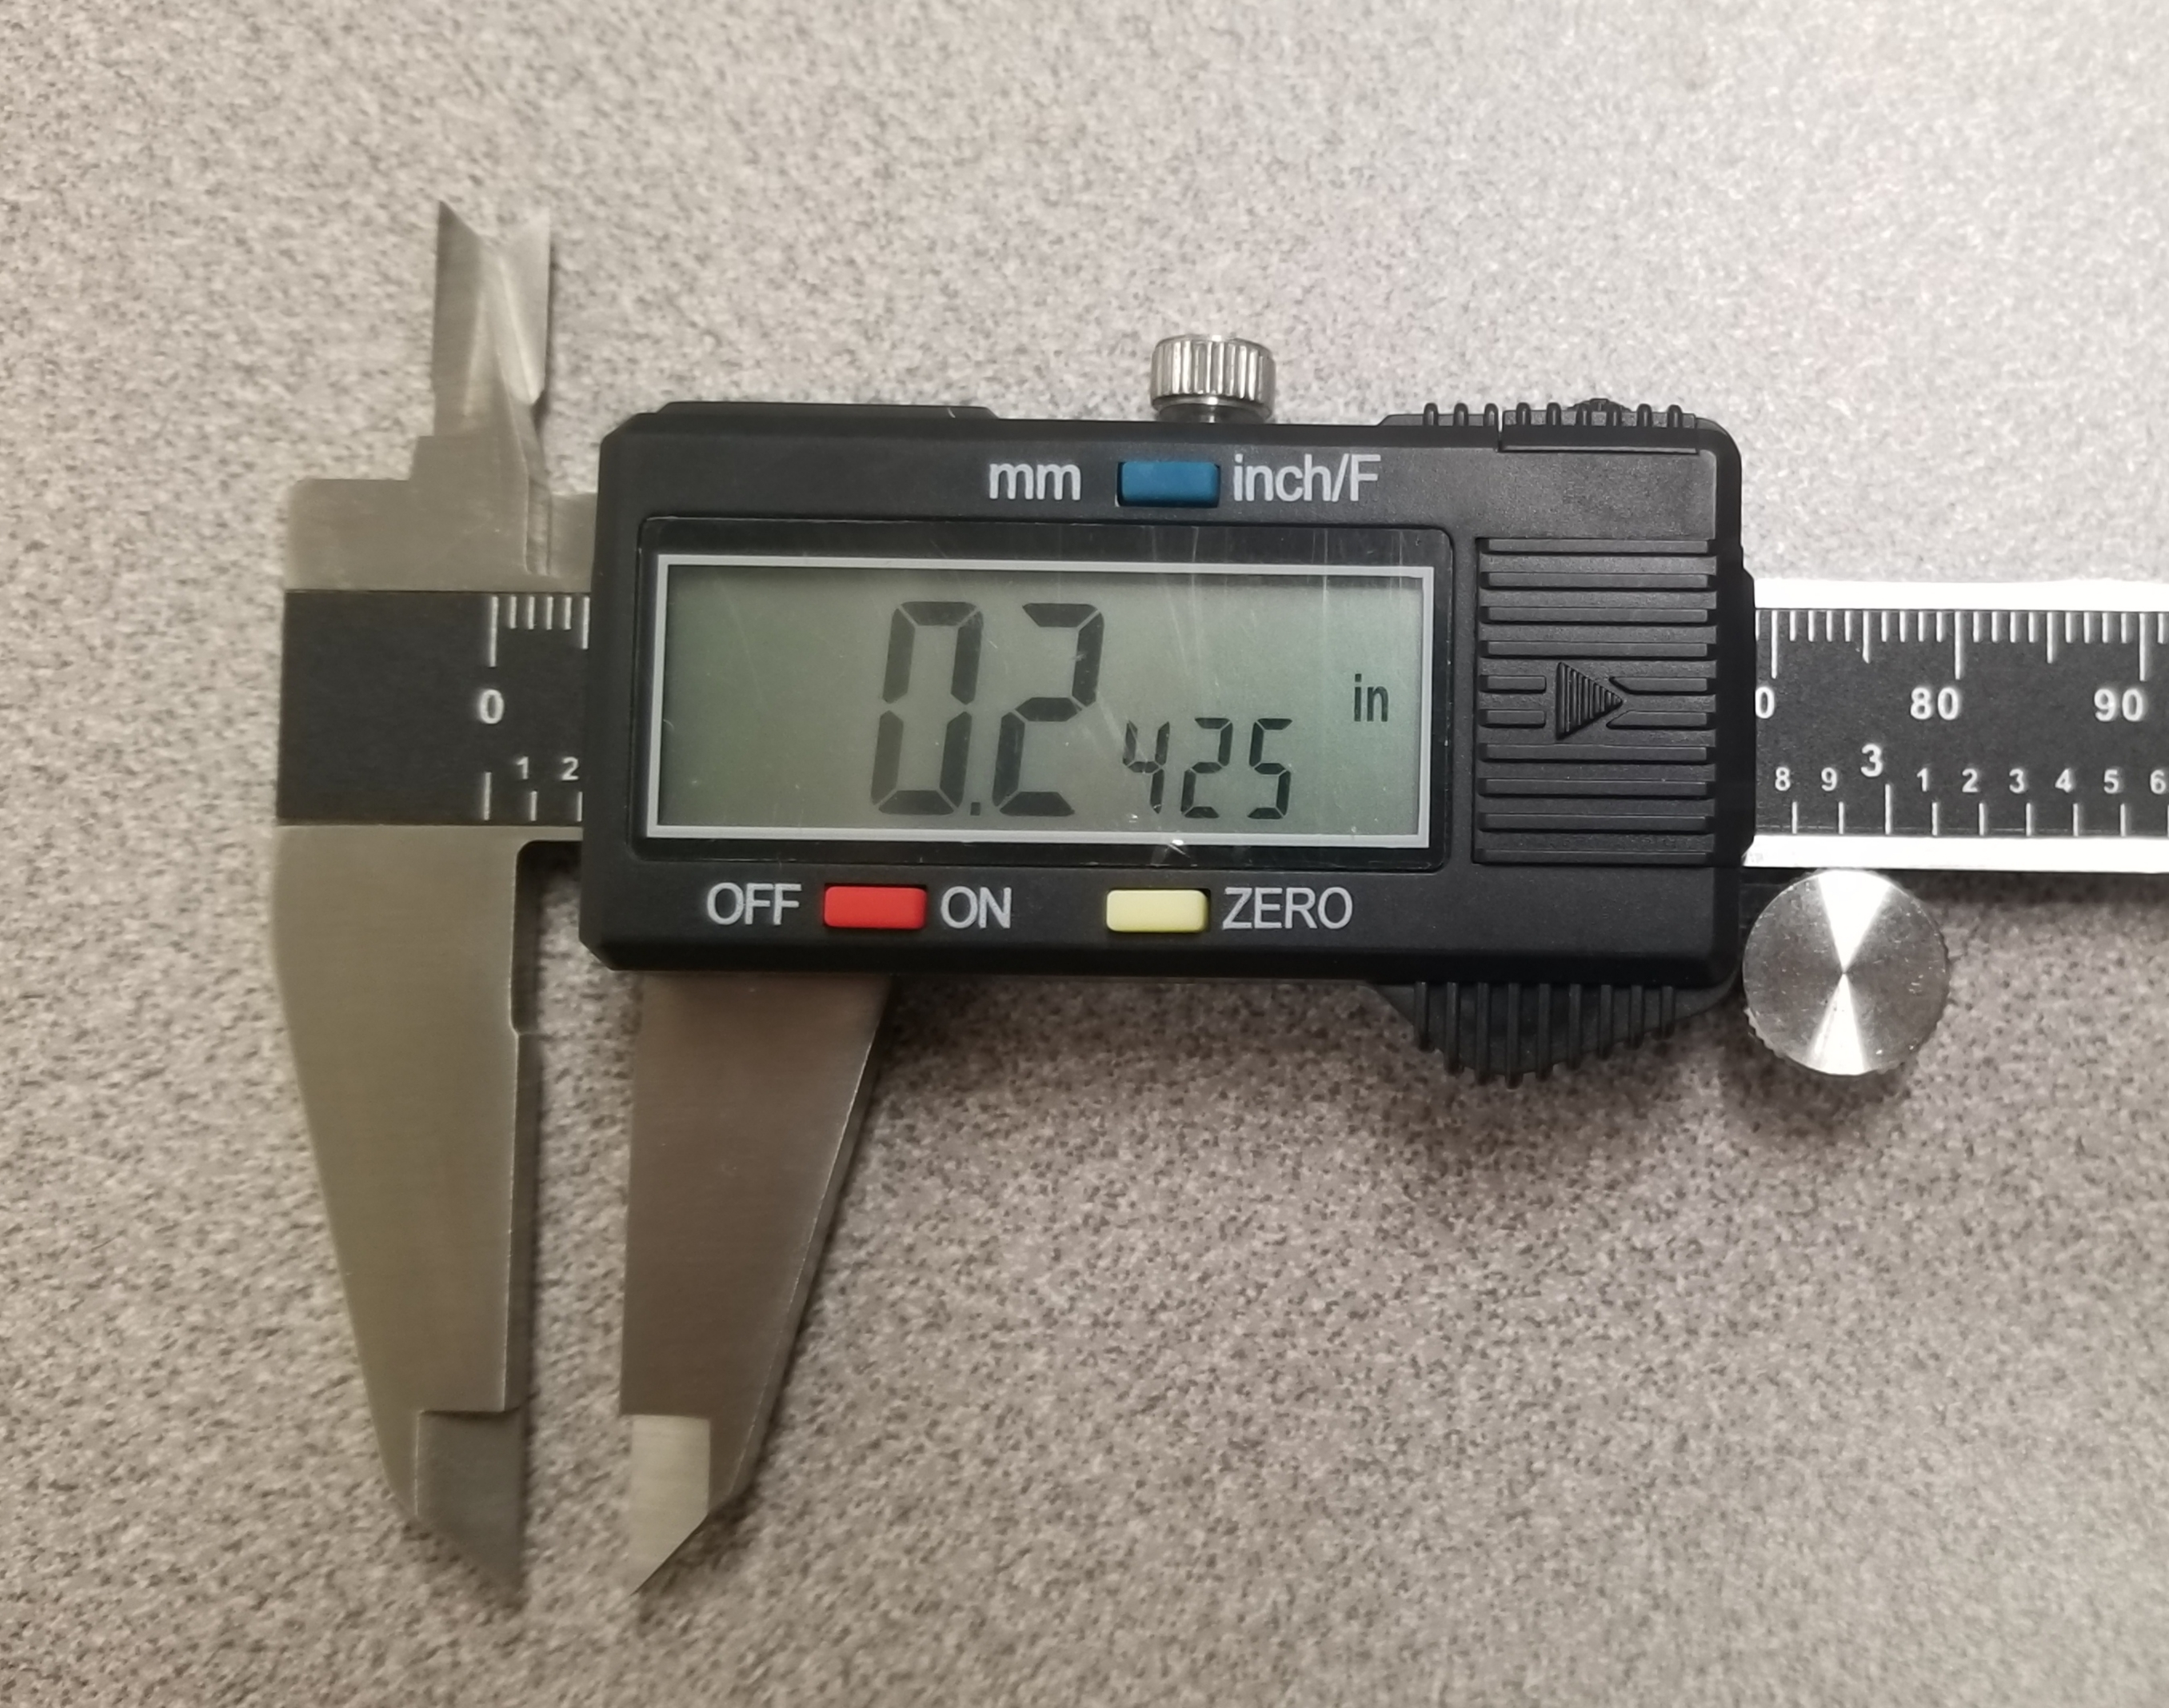
\includegraphics[scale=.25]{digital_calipers_fig2_cropped.png}
		\end{multicols}
	}

% Section V:
\section{\sectiontitleV}

	
	\frame{
		\frametitle{\sectiontitleIII}

			{\bf Activity:} Compare and Constast 

			Complete the compare and constrast acivities on the following two slides.

			{\bf Duration:} $\sim 10$ minutes

			{\bf Groups:} 2-3 members

			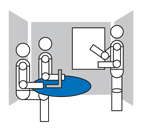
\includegraphics[scale=0.5]{Brainstorm_room.png}

			{\bf Deliverable:}  Each group member submit a separate copy of your work written in your own words. Include the names of all group members on submission.

	}


	\frame{
		\frametitle{\sectiontitleIII}

		Discuss three benefits and three shortcomings of a {\bf vernier calipers}. 

		\begin{multicols}{2}
		\underline{Pros}
		\begin{itemize}
		\item
		\item
		\item
		\end{itemize}
		\underline{Cons}
		\begin{itemize}
		\item 
		\item
		\item
		\end{itemize}
		\end{multicols}

	}


	\frame{
		\frametitle{\sectiontitleIV}

	     Discuss three benefits and three shortcomings of a {\bf digital calipers}. 


		\begin{multicols}{2}
		\underline{Pros}
		\begin{itemize}
		\item 
		\item
		\item
		\end{itemize}
		\underline{Cons}
		\begin{itemize}
		\item 
		\item
		\item
		\end{itemize}
		\end{multicols}

	}

\end{document}





